% Provenance (never printed): see sources/outline_sources.md (Year 1: the wind-driven
% circulation, gyres, Ekman transport and upwelling, western boundary currents, the
% meridional overturning circulation and the water masses). Exercise and problem values in
% the Book 3 scratch calculator calc/ch29.py; figures from figdata/bachelor-1/
% ekman_hodograph.py (Ekman's solution with Ekman's constants) and stommel_gyre.py
% (Stommel's 1948 model, exercise parameters), the world map from figdata/shared/geo.py.
% Physics owns the Coriolis force (recalled). Book 1 (g8) gave the surface currents and
% the gyres in words, Book 2 (g10) upwelling: re-founded here with the Ekman balance.
% Ch. 26 owns the T-S diagram and the water masses, ch. 28 the Coriolis parameter, the
% geostrophic wind and the mean meridional streamfunction. The Sverdrup balance, the
% vorticity argument and the derivation of the Ekman spiral are the Year 3 volume's; ENSO
% the Year 2 volume's.
\chapter{海洋环流}\label{ch:b1:ocean-circulation}

1992 年，北太平洋上的一场风暴中，一只集装箱从
一艘由香港驶往美国的货船上被冲入海中。集装箱破裂，
释放出约 \num{29000} 只橡胶鸭子和其他浴缸玩具，它们漂浮而去，走得很远；
其中部分玩具被发现的地点，帮助科学家了解了曾携带它们的洋流。
漂浮的玩具随表层海水运动，
而海洋的表层海水并非随意漂流：它在大洋盆地尺度上形成环流，
沿大洋西岸以狭窄的洋流向北奔涌，
并在少数选定的地方上升或下沉。本章
将解释风如何推动上层海洋运动，为何水流与风成直角，
为何最强的洋流紧贴大洋的西侧，
以及缓慢的翻转环流如何把水输送到深海并使之返回。
% ledger: noaa:floatees

\begin{omfigure}
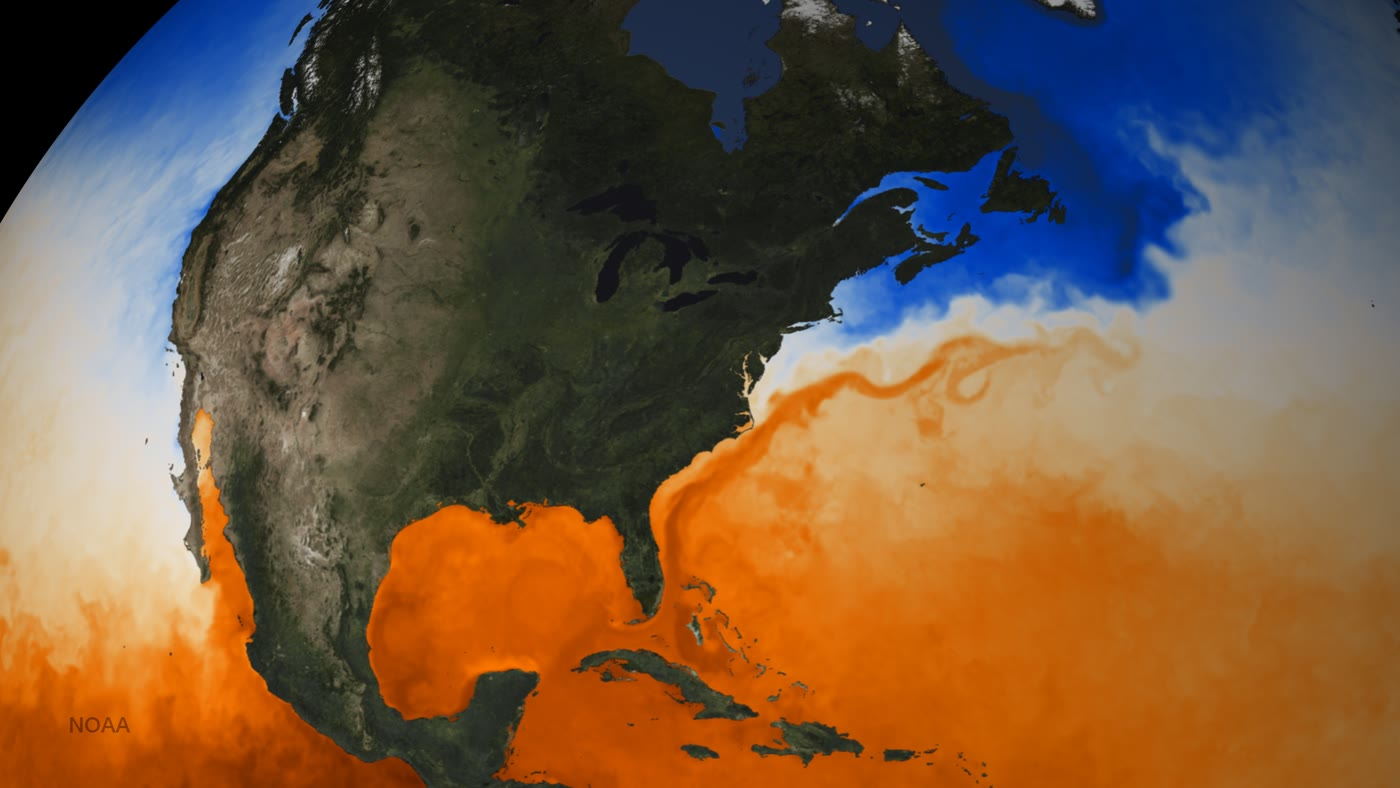
\includegraphics[width=0.85\linewidth]{images/book3/b1-gulf-stream-sst.jpg}

{\small 2016 年 6 月初北美周围的海表温度，
依据卫星数据绘制（暖水为橙色，冷水为蓝色）。墨西哥湾流
离开美国海岸，形成温暖而蜿蜒的水带，横穿
大西洋流向欧洲；在相同\omterm{def:b1:spherical-astronomy:geographic}{纬度}上，太平洋沿岸外的海水
明显比大西洋沿岸外的海水更冷。（NOAA、NESDIS，公有领域，经
维基共享资源。）}
\label{fig:b1:ocean-circulation:sst}
\end{omfigure}
% ledger: commons:gulf-stream-sst, noaa:gulf-stream-heat

\begin{recall}
物理各册给出了科里奥利力。在\Cref{ch:b1:atmospheric-circulation}
中，其水平部分写作 $-f\,\vec k\times\vec v$，
\omterm{def:b1:atmospheric-circulation:coriolis-parameter}{科里奥利参数} $f = 2\Omega\sin\varphi$（$\Omega = \qty{7.292e-5}{rad.s^{-1}}$），并由此得到
\omterm{def:b1:atmospheric-circulation:winds}{信风}（赤道至约 \ang{30} 之间的东风），
以及其外侧的\omterm{def:b1:atmospheric-circulation:winds}{西风带}；还定义了翻转环流的\omterm{def:b1:atmospheric-circulation:streamfunction}{平均经向流函数}。
在\Cref{ch:b1:fluid-envelopes-structure}中给出了\omterm{def:b1:fluid-envelopes-structure:ocean-layers}{混合层}与\omterm{def:b1:fluid-envelopes-structure:ocean-layers}{温跃层}、
海水密度、\omterm{def:b1:fluid-envelopes-structure:ts-diagram}{温盐图}以及南大西洋的\omterm{def:b1:fluid-envelopes-structure:ts-diagram}{水团}；
以及在\cref{ch:b1:radiation-heat-transport}中给出的由大气与
海洋共同承担的向极热量输送。第 1 册描述了表层洋流与大型环流；
第 2 册描述了沿某些海岸冷水的\omterm{def:b1:ocean-circulation:upwelling}{上升流}。
% ledger: earth:Trot, nos:gyres
\end{recall}

\section{风与表层洋流}\label{sec:b1:ocean-circulation:wind}

风通过摩擦推动海水。它的力分布在海面上，
并像压强一样，按单位面积来度量。

\begin{definition}[风应力]\label{def:b1:ocean-circulation:wind-stress}
\emph{风应力}\index{风应力} $\vec T$ 是风施加在海面上的单位面积水平力，
单位为帕斯卡。它是空气水平动量向海洋的向下传递，
方向近似沿风向。
其大小由体公式给出：
\[
  T = \rho_a C_D U_{10}^2,
\]
其中 $\rho_a = \qty{1.3}{kg.m^{-3}}$ 为空气密度，$U_{10}$ 为
海面以上 \qty{10}{m} 处的风速，$C_D$ 为无量纲的阻力系数。
\end{definition}
% ledger: stewart:wind-stress

阻力系数由快速仪器测得，这些仪器记录海浪上方几米处
风的湍流脉动。对于中性稳定的空气，
耶兰德和泰勒的测量给出
\[
  1000\,C_D = 0.29 + \frac{3.1}{U_{10}} + \frac{7.7}{U_{10}^2}
  \quad (\qtyrange{3}{6}{m/s}),
  \qquad
  1000\,C_D = 0.60 + 0.071\,U_{10}
  \quad (\qtyrange{6}{26}{m/s}),
\]
式中 $U_{10}$ 的单位为米每秒。风速为 \qty{10}{m/s} 时，$C_D =
\num{1.31e-3}$，应力为 $T = 1.3 \times \num{1.31e-3} \times 100 =
\qty{0.170}{Pa}$；风速为 \qty{5}{m/s} 时为 \qty{0.040}{Pa}；大
风（\qty{20}{m/s}）时为 \qty{1.05}{Pa}。风速由 \qty{10}{m/s} 增至 \qty{20}{m/s}，
应力增为 $6.2$ 倍，而非 $4$ 倍：较粗糙的海面对风的拖拽更强。这些
应力非常微小，约为大气压强的百万分之一，但它们不停歇地作用于
整个海洋。
% ledger: stewart:drag-coefficient (computed in figdata/bachelor-1/ekman_hodograph.py and calc/ch29.py)

应力的分布跟随风场的分布。在热带的\omterm{def:b1:atmospheric-circulation:winds}{信风}（向西吹）
与中\omterm{def:b1:spherical-astronomy:geographic}{纬度}的\omterm{def:b1:atmospheric-circulation:winds}{西风带}（向东吹）之间，各大洋盆地的表层海水
被带动而旋转起来。

\begin{definition}[环流；副热带环流与副极地环流]\label{def:b1:ocean-circulation:gyre}
\emph{环流}\index{环流}是充满一个大洋盆地的
大型旋转洋流系统。\emph{副热带环流}\index{副热带环流}位于\omterm{def:b1:atmospheric-circulation:winds}{信风}
与\omterm{def:b1:atmospheric-circulation:winds}{西风带}之间，在北半球沿顺时针方向转动，
在南半球沿逆时针方向转动。\emph{副极地环流}\index{副极地环流}位于
\omterm{def:b1:atmospheric-circulation:winds}{西风带}的极向一侧，转向相反。
\end{definition}
% ledger: nos:gyre-def, nos:boundary-currents, stewart:north-atlantic

\omterm{def:b1:ocean-circulation:gyre}{副热带环流}共有五个，分别位于北大西洋、南大西洋、
北太平洋、南太平洋和印度洋；没有一个跨越赤道。在北大西洋，
\omterm{def:b1:ocean-circulation:gyre}{副热带环流}西侧由沿美国海岸的墨西哥湾流闭合，
东侧由非洲外海的加那利洋流闭合；其北侧
为\omterm{def:b1:ocean-circulation:gyre}{副极地环流}，逆时针转动，其南侧为北大西洋暖流，
其西侧为向南流动的拉布拉多洋流。在低\omterm{def:b1:spherical-astronomy:geographic}{纬度}，
大西洋和太平洋中向西流动的赤道洋流被
一支向东流动的赤道逆流隔开。环流并不对称：每个\omterm{def:b1:ocean-circulation:gyre}{副热带环流}都
由位于其盆地西侧的强而窄的洋流闭合，
东侧则由弱而宽的洋流闭合。在南极洲周围，没有大陆阻挡，
南极绕极流沿地球向东绕行，由
南大洋的\omterm{def:b1:atmospheric-circulation:winds}{西风带}驱动。
% ledger: nos:boundary-currents, stewart:north-atlantic, stewart:heat-conveyor, lien:kuroshio, donohue:acc, stewart:acc

\begin{omfigure}
\begin{tikzpicture}
\begin{axis}[ommap, width=0.98\linewidth, xtick={-180,-120,...,180}, ytick={-60,-30,0,30,60}]
% land: figdata/shared/geo.py; ledger: data:ne-land. Arrows placed by hand from the
% ledgered pattern: nos:boundary-currents, stewart:north-atlantic, lien:kuroshio,
% donohue:acc, stewart:acc
\addplot[fill=omLithAlluv, draw=black!45, line width=0.2pt, forget plot] table {figdata/out/shared-geo-land.dat};
% North Atlantic subtropical gyre (clockwise)
\addplot[omThm, line width=1.1pt, -{Stealth[length=4pt]}, smooth] coordinates {(-80,26) (-77,32) (-70,37) (-58,40) (-44,41)};
\addplot[omThm, line width=1.1pt, -{Stealth[length=4pt]}, smooth] coordinates {(-38,40) (-28,39) (-20,36)};
\addplot[omThm, line width=1.1pt, -{Stealth[length=4pt]}, smooth] coordinates {(-19,32) (-21,24) (-26,17)};
\addplot[omThm, line width=1.1pt, -{Stealth[length=4pt]}, smooth] coordinates {(-32,14) (-45,13) (-60,15)};
% North Atlantic subpolar gyre (anticlockwise)
\addplot[omDef, line width=1.1pt, -{Stealth[length=4pt]}, smooth] coordinates {(-40,47) (-28,52) (-18,57)};
\addplot[omDef, line width=1.1pt, -{Stealth[length=4pt]}, smooth] coordinates {(-24,61) (-35,62) (-44,59)};
\addplot[omDef, line width=1.1pt, -{Stealth[length=4pt]}, smooth] coordinates {(-55,59) (-56,53) (-51,47)};
% North Pacific subtropical gyre (clockwise)
\addplot[omThm, line width=1.1pt, -{Stealth[length=4pt]}, smooth] coordinates {(123,19) (125,26) (133,32) (143,36) (156,38)};
\addplot[omThm, line width=1.1pt, smooth] coordinates {(162,39) (172,40) (180,40.5)};
\addplot[omThm, line width=1.1pt, -{Stealth[length=4pt]}, smooth] coordinates {(-180,40.5) (-165,41) (-148,40)};
\addplot[omThm, line width=1.1pt, -{Stealth[length=4pt]}, smooth] coordinates {(-133,37) (-128,29) (-122,20)};
\addplot[omThm, line width=1.1pt, -{Stealth[length=4pt]}, smooth] coordinates {(-125,13) (-150,12) (-175,13)};
\addplot[omThm, line width=1.1pt, -{Stealth[length=4pt]}, smooth] coordinates {(170,13) (152,14) (135,15)};
% South Atlantic subtropical gyre (anticlockwise)
\addplot[omThm, line width=1.1pt, -{Stealth[length=4pt]}, smooth] coordinates {(2,-8) (-15,-9) (-30,-9)};
\addplot[omThm, line width=1.1pt, -{Stealth[length=4pt]}, smooth] coordinates {(-34,-14) (-39,-24) (-47,-34)};
\addplot[omThm, line width=1.1pt, -{Stealth[length=4pt]}, smooth] coordinates {(-42,-40) (-20,-40) (2,-38)};
\addplot[omThm, line width=1.1pt, -{Stealth[length=4pt]}, smooth] coordinates {(10,-31) (9,-23) (6,-15)};
% South Pacific subtropical gyre (anticlockwise)
\addplot[omThm, line width=1.1pt, -{Stealth[length=4pt]}, smooth] coordinates {(-88,-10) (-120,-11) (-160,-12)};
\addplot[omThm, line width=1.1pt, -{Stealth[length=4pt]}, smooth] coordinates {(160,-16) (157,-26) (162,-35)};
\addplot[omThm, line width=1.1pt, -{Stealth[length=4pt]}, smooth] coordinates {(-170,-40) (-140,-41) (-105,-39)};
\addplot[omThm, line width=1.1pt, -{Stealth[length=4pt]}, smooth] coordinates {(-82,-36) (-82,-27) (-85,-17)};
% Indian Ocean subtropical gyre (anticlockwise)
\addplot[omThm, line width=1.1pt, -{Stealth[length=4pt]}, smooth] coordinates {(98,-13) (80,-14) (60,-15)};
\addplot[omThm, line width=1.1pt, -{Stealth[length=4pt]}, smooth] coordinates {(47,-22) (40,-29) (33,-34)};
\addplot[omThm, line width=1.1pt, -{Stealth[length=4pt]}, smooth] coordinates {(50,-38) (75,-37) (100,-35)};
\addplot[omThm, line width=1.1pt, -{Stealth[length=4pt]}, smooth] coordinates {(108,-31) (106,-24) (102,-18)};
% Antarctic Circumpolar Current (eastward)
\addplot[omMeth, line width=1.4pt, -{Stealth[length=5pt]}, smooth] coordinates {(-62,-58) (-40,-55) (-15,-52)};
\addplot[omMeth, line width=1.4pt, -{Stealth[length=5pt]}, smooth] coordinates {(5,-52) (40,-50) (75,-50)};
\addplot[omMeth, line width=1.4pt, -{Stealth[length=5pt]}, smooth] coordinates {(95,-51) (130,-53) (165,-56)};
\addplot[omMeth, line width=1.4pt, -{Stealth[length=5pt]}, smooth] coordinates {(-170,-58) (-130,-59) (-85,-59)};
\node[font=\scriptsize, anchor=west, fill=white, fill opacity=0.8, text opacity=1, inner sep=1pt] at (axis cs:-66,31) {墨西哥湾流};
\node[font=\scriptsize, anchor=west, fill=white, fill opacity=0.8, text opacity=1, inner sep=1pt] at (axis cs:-11,25) {加那利};
\node[font=\scriptsize, anchor=east, fill=white, fill opacity=0.8, text opacity=1, inner sep=1pt] at (axis cs:-58,52) {拉布拉多};
\node[font=\scriptsize, anchor=west, fill=white, fill opacity=0.8, text opacity=1, inner sep=1pt] at (axis cs:142,28) {黑潮};
\node[font=\scriptsize, anchor=north, fill=white, fill opacity=0.8, text opacity=1, inner sep=1pt] at (axis cs:-150,9) {北赤道};
\node[font=\scriptsize, anchor=north, fill=white, fill opacity=0.8, text opacity=1, inner sep=1pt] at (axis cs:0,-62) {南极绕极流};
\end{axis}
\end{tikzpicture}

{\small 表层海洋的环流（陆地地图上的示意箭头）。
深红色：五个\omterm{def:b1:ocean-circulation:gyre}{副热带环流}，北半球顺时针、
南半球逆时针，每个环流都有一条狭窄的\omterm{def:b1:ocean-circulation:wbc}{西边界流}；蓝色：
北大西洋\omterm{def:b1:ocean-circulation:gyre}{副极地环流}；绿色：南极绕极流。
图中仅标出正文讨论的洋流。箭头表示
流动的方向，而非其速率。}
\label{fig:b1:ocean-circulation:gyres}
\end{omfigure}
% ledger: data:ne-land, nos:boundary-currents, stewart:north-atlantic, lien:kuroshio, donohue:acc

这一格局有两点需要解释。第一是旋转的方向：
在\omterm{def:b1:ocean-circulation:gyre}{副热带环流}靠赤道的一侧，\omterm{def:b1:atmospheric-circulation:winds}{信风}向西吹，
但环流中的洋流并不简单地顺着风流动，表层水
与风向成一定夹角漂移。第二是不对称性：环流的回流
被挤压在盆地的西侧。两者都源于
地球的自转。

\section{埃克曼输送}\label{sec:b1:ocean-circulation:ekman}

\begin{history}[南森与埃克曼，1898--1905]
弗里德约夫·南森在北极考察期间注意到，风驱动
海冰并非沿风向运动，而是以 \ang{20} 至 \ang{40} 的夹角偏向其
右侧（顺风向看去）。他推断，运动的冰上
有三个力必须平衡：风的推力、水的摩擦力和科里奥利力。他
请气象学家维尔海姆·皮叶克尼斯安排一名学生研究
地球自转对风生洋流的影响。这名学生
瓦尔弗里德·埃克曼在乌普萨拉大学撰写博士论文时建立了理论，并
于 1905 年加以推广。他的解至今仍是风生
海洋理论的出发点。
\end{history}
% ledger: stewart:ekman-layer, nos:ekman-spiral

\begin{definition}[埃克曼层、埃克曼输送、埃克曼螺旋]\label{def:b1:ocean-circulation:ekman}
\emph{埃克曼层}\index{埃克曼层}是海洋中一层很薄的表层，
厚度至多几百米，\omterm{def:b1:ocean-circulation:wind-stress}{风应力}通过湍流摩擦向下传递，
并与科里奥利力相平衡。\emph{埃克曼
输送}\index{埃克曼输送}是该层每秒穿过
一个竖直条带（宽 \qty{1}{m}、自表面向下直至层底以下）的水的
质量：
\[
  \vec M = \int_{-d}^{0} \rho\,\vec v\,\mathrm dz \quad (\unit{kg.m^{-1}.s^{-1}});
\]
除以密度，即得每米的体积输送，单位为
\unit{m^2.s^{-1}}。\emph{埃克曼螺旋}\index{埃克曼螺旋}是
洋流随深度在该层中转向并减弱。海洋输送量以
\emph{斯韦德鲁普}\index{斯韦德鲁普（单位）}为单位：\qty{1}{\sverdrup} $=
\qty{e6}{m^3.s^{-1}}$。
\end{definition}
% ledger: stewart:ekman-layer, stewart:ekman-transport

\begin{theorem}[埃克曼输送]\label{thm:b1:ocean-circulation:ekman}
在稳态下，远离海岸、水深远大于\omterm{def:b1:ocean-circulation:ekman}{埃克曼层}时，
\omterm{def:b1:ocean-circulation:ekman}{埃克曼输送}仅取决于\omterm{def:b1:ocean-circulation:wind-stress}{风应力} $\vec T$ 和\omterm{def:b1:atmospheric-circulation:coriolis-parameter}{科里奥利
参数} $f$：
\[
  \vec M = \frac{1}{f}\,\vec T\times\vec k,
  \qquad |\vec M| = \frac{|\vec T|}{|f|}.
\]
它与\omterm{def:b1:ocean-circulation:wind-stress}{风应力}垂直，北半球位于其右侧，
南半球位于其左侧。
\end{theorem}
% ledger: stewart:ekman-transport

\begin{proof}
设 $\vec\tau(z)$ 为水层中 $z$ 以上的水对其下方水体施加的水平应力。
在表面，它即为\omterm{def:b1:ocean-circulation:wind-stress}{风应力}，$\vec\tau(0) =
\vec T$；在层底之下，风驱动的流动已衰减，
它为零，$\vec\tau(-d) = \vec 0$。取位于 $z$ 与 $z + \mathrm dz$ 之间的\omterm{def:b1:field-lab-methods-1:thin-section}{薄片}，
水平面积为单位面积，其顶面受 $\vec\tau(z + \mathrm dz)$，
底面受 $-\vec\tau(z)$：净摩擦力为 $(\partial\vec
\tau/\partial z)\,\mathrm dz$。其质量为 $\rho\,\mathrm dz$，所受水平
科里奥利力为 $-f\,\vec k\times\vec v\,\rho\,\mathrm dz$。在稳态下，
水平方向上各处无变化，二者平衡：
\[
  -f\rho\,\vec k\times\vec v + \frac{\partial\vec\tau}{\partial z} = \vec 0 .
\]
从 $-d$ 到 $0$ 积分，
\[
  -f\,\vec k\times\vec M + \vec\tau(0) - \vec\tau(-d) = \vec 0,
  \qquad\text{即}\qquad \vec k\times\vec M = \frac{\vec T}{f}.
\]
对水平矢量有 $\vec k\times(\vec k\times\vec M) = -\vec M$；
两边左乘 $\vec k\times$，得 $-\vec M = \vec k\times\vec T/f$，故 $\vec M =
\vec T\times\vec k/f$。矢量 $\vec T\times\vec k$ 是将 $\vec T$
自上方俯视顺时针旋转 \ang{90} 所得：$f > 0$ 时位于风的右侧，
$f < 0$ 时位于左侧。其大小为 $|\vec T|$。
\end{proof}

该结果不依赖于层内摩擦如何起作用，而这一点
尚不清楚：只有顶部应力及其在底部的消失进入结果。
因此，输送量远比速度本身稳健。整个水层的水合在一起，
沿与风垂直的方向运动，这一结论初看颇为奇特，
但只要想到在一天或更长时间内，科里奥利力有足够的时间
使每一股流动都发生偏转，便不难理解。

\begin{example}[清劲风下的输送]\label{ex:b1:ocean-circulation:transport}
一股风速为 \qty{10}{m/s}、向北吹的风，在北纬 \ang{35} 处施加
$T = \qty{0.170}{Pa}$。取 $f = 2\Omega\sin\ang{35} = \qty{8.365e-5}{s^{-1}}$，
则\omterm{def:b1:ocean-circulation:ekman}{埃克曼输送}为 $0.170/(\num{8.365e-5}) = \qty{2036}{kg.m^{-1}.s^{-1}}$，方向向东。
取 $\rho = \qty{1027}{kg.m^{-3}}$，则每横跨输送方向一米的输送量为 \qty{1.98}{m^3.s^{-1}}，
对于长 \qty{1000}{km} 的横截线，约为
\qty{2}{\sverdrup}。
\end{example}
% ledger: stewart:drag-coefficient, stewart:ekman-constants, earth:Trot (computed in calc/ch29.py)

该定理已在海上得到检验。在大西洋北纬 \ang{11} 处，\omterm{def:b1:atmospheric-circulation:winds}{信风}向西吹，
\omterm{def:b1:ocean-circulation:ekman}{埃克曼输送}向北；用海流剖面仪直接测得，
其值为
\qty[uncertainty-mode=separate]{12.0 \pm 5.5}{\sverdrup}，与之相比，
由考察期间测得风计算所得的值为
\qty[uncertainty-mode=separate]{8.8 \pm 1.9}{\sverdrup}，
由多年平均风得出的值为
\qty[uncertainty-mode=separate]{13.5 \pm 0.3}{\sverdrup}。
% ledger: stewart:ekman-transport

层内流动随深度的分布取决于
摩擦。埃克曼采用了最简单的模型：湍流摩擦与流动的
竖直剪切成正比，$\vec\tau = \rho A_z\,\partial\vec v/\partial z$，其中
涡动黏度 $A_z$ 为常数。

\begin{proposition}[埃克曼螺旋]\label{prop:b1:ocean-circulation:spiral}
对于指向北方的稳定\omterm{def:b1:ocean-circulation:wind-stress}{风应力} $T$，作用于北半球一片
深水、均匀的海洋上，取常值涡动黏度 $A_z$，高度 $z
\leq 0$ 处的流动为
\[
  u = V_0\,e^{az}\cos\Bigl(\frac\pi4 + az\Bigr),\qquad
  v = V_0\,e^{az}\sin\Bigl(\frac\pi4 + az\Bigr),\qquad
  a = \sqrt{\frac{f}{2A_z}},\quad V_0 = \frac{T}{\rho\sqrt{fA_z}},
\]
其中 $u$ 向东，$v$ 向北。在表面，流动方向与风向成 \ang{45} 角，偏于
风的右侧；随深度增加，速度按 $e^{az}$ 减弱，
且向右进一步偏转。在深度 $D_E = \pi/a$（即埃克曼深度）处，其流向与表面流动相反，
其速度为表面速度的 $e^{-\pi} = \num{0.043}$ 倍。
\end{proposition}
\admitted
% ledger: stewart:ekman-solution

该推导求解上文证明中平衡关系的两个方程 $f v + A_z u'' = 0$ 与 $-f u + A_z v'' =
0$ 为上文证明中的平衡关系；其详细推导在本科三年级分册中给出，并且
\cref{exo:b1:ocean-circulation:10} 检验这些公式满足方程，
并且螺旋恰好输送定理所给的输送量。要使用该螺旋，
需要 $A_z$，而它无法直接测量。埃克曼收集了
表面流动速度的观测数据，并对 $|\varphi| \geq \ang{10}$ 得到
\[
  V_0 = \frac{0.0127\,U_{10}}{\sqrt{\sin|\varphi|}},
  \qquad\text{由此得到}\qquad
  D_E = \frac{7.6\,U_{10}}{\sqrt{\sin|\varphi|}},
\]
单位为国际单位制，其中他的阻力系数 $C_D = \num{2.6e-3}$，且 $\rho_a =
\qty{1.25}{kg.m^{-3}}$。在北纬 \ang{35} 处，风速为 \qty{10}{m/s} 时，$D_E =
\qty{100}{m}$，$V_0 = \qty{0.17}{m/s}$；\omterm{def:b1:ocean-circulation:ekman}{埃克曼层}的厚度约为
\qty{45}{m}（中\omterm{def:b1:spherical-astronomy:geographic}{纬度}微风下）至热带大风下的 \qty{300}{m}，
并且表面流动速度为风速的 \qtyrange{1}{2.5}{\percent}。
% ledger: stewart:ekman-constants (computed in figdata/bachelor-1/ekman_hodograph.py)

\begin{omfigure}
\begin{tikzpicture}
\begin{axis}[ompt, name=hodo, width=0.5\linewidth, axis equal image, xmin=-6, xmax=22,
  ymin=-6, ymax=17, xlabel={向东流动速度（\unit{cm/s}）}, ylabel={向北流动速度（\unit{cm/s}）},
  xtick={-5,0,5,10,15,20}, ytick={-5,0,5,10,15}]
% figdata/bachelor-1/ekman_hodograph.py; ledger: stewart:ekman-solution, stewart:ekman-constants
\addplot[black!45, line width=0.6pt] table[x expr=\thisrow{u}*100, y expr=\thisrow{v}*100] {figdata/out/bachelor-1-ekman_hodograph-tips.dat};
\addplot[omDef, line width=0.6pt, -{Stealth[length=3pt]}, quiver={u=\thisrow{u}*100, v=\thisrow{v}*100}]
  table[x expr=0, y expr=0] {figdata/out/bachelor-1-ekman_hodograph-arrows.dat};
\draw[omThm, line width=1.6pt, -{Stealth[length=6pt]}] (axis cs:-3,0) -- (axis cs:-3,14);
\node[font=\scriptsize, text=omThm, anchor=west] at (axis cs:-2.6,13) {风};
\draw[omMeth, line width=1.6pt, -{Stealth[length=6pt]}] (axis cs:0,-3.2) -- (axis cs:16,-3.2);
\node[font=\scriptsize, text=omMeth, anchor=north] at (axis cs:8,-3.6) {埃克曼输送};
\node[font=\scriptsize, anchor=south west] at (axis cs:11.9,11.9) {表面};
\node[font=\scriptsize, anchor=north east] at (axis cs:-0.3,-0.4) {$D_E$};
\end{axis}
\begin{axis}[ompt, at={(hodo.east)}, anchor=west, xshift=1.4cm, width=0.42\linewidth, height=6.2cm,
  xmin=-4, xmax=14, ymin=-200, ymax=0, xlabel={流动速度（\unit{cm/s}）}, ylabel={深度（\unit{m}）},
  yticklabel={$\pgfmathprintnumber[fixed]{\tick}$},
  legend style={font=\scriptsize, at={(0.97,0.03)}, anchor=south east, cells={anchor=west}}]
\addplot[black!40, forget plot] coordinates {(0,-200) (0,0)};
\addplot[omDef, line width=1pt] table[x expr=\thisrow{u}*100, y=z] {figdata/out/bachelor-1-ekman_hodograph-profile.dat};
\addlegendentry{向东}
\addplot[omProp, line width=1pt, dashed] table[x expr=\thisrow{v}*100, y=z] {figdata/out/bachelor-1-ekman_hodograph-profile.dat};
\addlegendentry{向北}
\addplot[black!50, densely dotted, forget plot] coordinates {(-4,-100.35) (14,-100.35)};
\node[font=\scriptsize, anchor=south east] at (axis cs:13.8,-100.35) {$D_E = \qty{100}{m}$};
\end{axis}
\end{tikzpicture}

{\small 北纬 \ang{35} 处、风速为 \qty{10}{m/s}、向北吹的风作用下的\omterm{def:b1:ocean-circulation:ekman}{埃克曼螺旋}，
采用埃克曼常数。左图：自上方俯视所见的表层
及每隔十分之一埃克曼深度 $D_E$ 直至 $D_E$ 处的流（蓝色箭头），
灰色曲线连接其箭头末端；表层流位于风向右侧 \ang{45}，
深层流较弱且更偏右。整个层的输送（绿色；仅示方向）
位于风向右侧 \ang{90}。
右图：两个分量随深度的变化。}
\label{fig:b1:ocean-circulation:spiral}
\end{omfigure}
% ledger: stewart:ekman-solution, stewart:ekman-constants

螺旋是一种理想化的模型。来自系泊潜标上的海流计，
以及 1987 年至 1994 年间在太平洋中跟踪的 1503 个漂流浮标的测量表明，
在多日平均之后，流动与埃克曼理论吻合得相当好：层的深度几乎就是他给出的
$7.12\,U_{10}/\sqrt{\sin|\varphi|}$；表层流约为
约为他的理论值的一半；风与表层流之间的夹角在中\omterm{def:b1:spherical-astronomy:geographic}{纬度}处接近
\ang{45}；输送位于风向右侧 \ang{90}。
在数小时的时间尺度上，图像会被惯性振荡模糊，而平衡
的建立需要风持续吹上一两天。
% ledger: stewart:ekman-observed

\section{上升流与埃克曼抽吸}\label{sec:b1:ocean-circulation:upwelling}

若\omterm{def:b1:ocean-circulation:ekman}{埃克曼输送}在各处不相同，则水在某些地方堆积，
在另一些地方被带走；这一差额由竖直运动来补偿。

\begin{definition}[上升流、下降流、沿岸上升流]\label{def:b1:ocean-circulation:upwelling}
\emph{上升流}\index{上升流}是下方的水上升进入海洋表层的运动，
以补充被带走的表层水；\emph{下降流}%
\index{下降流}是表层水在其堆积处下沉的运动。
\emph{沿岸上升流}\index{沿岸上升流}出现于沿海岸吹的风驱动\omterm{def:b1:ocean-circulation:ekman}{埃克曼输送}
离开海岸的情形：在北半球，
即海岸位于风左侧的风。
\end{definition}
% ledger: noaa:upwelling, stewart:upwelling

\begin{proposition}[沿岸上升流]\label{prop:b1:ocean-circulation:coastal}
沿长为 $L$ 的平直海岸，\omterm{def:b1:ocean-circulation:wind-stress}{风应力}沿海岸的分量为 $T_\parallel$，
且其方向使\omterm{def:b1:ocean-circulation:ekman}{埃克曼输送}指向离岸，
则从\omterm{def:b1:ocean-circulation:ekman}{埃克曼层}下方抽升上来的体积为
\[
  Q = \frac{T_\parallel\,L}{\rho\,|f|}
\]
每秒。
\end{proposition}
% ledger: stewart:upwelling, stewart:ekman-transport

\begin{proof}
由\cref{thm:b1:ocean-circulation:ekman}，穿越海岸的输送
由沿岸的应力分量产生，其大小为每米海岸 $T_\parallel/|f|$；
故每秒沿离岸方向穿过与海岸平行的线的水量为 $T_\parallel L/(\rho|f|)$
立方米。在海岸本身处，
水无法穿越。处于稳态时，海岸与该线之间水的质量
不变：从表层离开的水必须从下方补充，
经由\omterm{def:b1:ocean-circulation:ekman}{埃克曼层}的底部进入。
\end{proof}

\begin{omfigure}
\begin{tikzpicture}[>={Stealth[length=2.2mm]}, font=\scriptsize]
% plan view
\begin{scope}
  \fill[omSea] (0,0) rectangle (3.2,4.2);
  \fill[omLithAlluv] (3.2,0) -- (3.2,4.2) -- (4.2,4.2) -- (4.2,0) -- cycle;
  \draw[black!60] (3.2,0) -- (3.2,4.2);
  \node[rotate=90] at (3.75,2.1) {陆地};
  \draw[omThm, line width=1.4pt, ->] (2.5,3.6) -- (2.5,1.4);
  \node[omThm, anchor=east] at (2.42,2.6) {风};
  \draw[omMeth, line width=1.4pt, ->] (2.2,0.9) -- (0.4,0.9);
  \node[omMeth, anchor=south, align=center] at (1.3,0.95) {埃克曼 \\输送};
  \draw[line width=0.8pt, ->] (0.4,3.3) -- (0.4,4.0) node[above, inner sep=1pt] {北};
  \node[anchor=north] at (2.1,-0.1) {俯视图};
\end{scope}
% cross-section, looking north: west on the left, east on the right
\begin{scope}[xshift=5.2cm]
  \fill[omSea] (0,-3.6) rectangle (8.0,0);
  \fill[omSea!70!blue!35] (0,-0.9) rectangle (8.0,0);
  \fill[omLithAlluv] (8.6,0.5) -- (8.6,-3.6) -- (5.4,-3.6) -- (7.2,-1.2) -- (8.0,0) -- (8.3,0.3) -- cycle;
  \draw[black!60] (5.4,-3.6) -- (7.2,-1.2) -- (8.0,0) -- (8.3,0.3);
  \draw[black!50] (0,0) -- (8.0,0);
  % isotherms rising towards the coast
  \foreach \y/\t in {-1.5/{暖}, -2.2/{}, -2.9/{冷}} {
    \draw[omDef, densely dashed] (0,\y) .. controls (3.5,\y) and (5.6,\y+0.7) .. (6.7,\y+1.15);
  }
  \node[anchor=west, text=omDef] at (0.05,-1.85) {等温线};
  \draw[omMeth, line width=1.4pt, ->] (6.0,-0.45) -- (1.0,-0.45);
  \node[omMeth, anchor=south] at (3.5,-0.42) {埃克曼输送，离岸};
  \node[anchor=north west] at (0.05,-0.92) {埃克曼层};
  \draw[omThm, line width=1.2pt, ->] (4.6,-2.9) .. controls (6.2,-2.6) and (6.8,-1.6) .. (7.25,-0.55);
  \node[omThm, anchor=east, align=right, fill=omSea, inner sep=1pt] at (4.5,-2.7) {冷而富营养 \\的水上升};
  \draw[omThm, line width=1pt] (6.3,0.85) circle (0.17);
  \fill[omThm] (6.3,0.85) circle (0.05);
  \node[omThm, anchor=east] at (6.05,0.85) {风指向观察者（南）};
  \fill[black!15] (7.5,1.1) ellipse (0.55 and 0.18);
  \fill[black!15] (8.0,1.2) ellipse (0.45 and 0.16);
  \node[anchor=south] at (7.8,1.3) {雾，低云};
  \node[anchor=north] at (0.2,-3.65) {西};
  \node[anchor=north] at (8.4,-3.65) {东};
  \node[anchor=north] at (4.2,-3.65) {剖面图，朝北看};
\end{scope}
\end{tikzpicture}

{\small 北半球海洋东岸的\omterm{def:b1:ocean-circulation:upwelling}{沿岸上升流}，
（示意图，深度未按比例）。左图：向南吹的风，
沿南–北\omterm{def:b1:geological-maps:attitude}{走向}的海岸，陆地位于东侧；\omterm{def:b1:ocean-circulation:ekman}{埃克曼
输送}位于风向右侧 \ang{90}，即离岸。右图：同一情形的
竖直剖面；\omterm{def:b1:ocean-circulation:ekman}{埃克曼层}中被带离岸边的水由下方补充，
等温线向海岸抬升，表面的冷水使其上方的空气
变冷。}
\label{fig:b1:ocean-circulation:upwelling}
\end{omfigure}
% ledger: stewart:upwelling, noaa:upwelling

在加利福尼亚外海，夏季风沿海岸向南吹，
情形与图中完全一致。上升的
水来自\omterm{def:b1:fluid-envelopes-structure:ocean-layers}{混合层}以下：它比表层水更冷，并且
营养物质更丰富。营养物质滋养浮游植物，浮游植物又滋养
浮游动物和鱼类：秘鲁、加利福尼亚、索马里、
摩洛哥和纳米比亚近海的\omterm{def:b1:ocean-circulation:upwelling}{上升流}区，支撑着世界主要渔业的一部分。冷水还
改变海岸的天气：流经其上的空气从下方被冷却，并
变为\omterm{def:b1:fluid-envelopes-structure:stability}{稳定层结}，此类海岸往往多雾和低层层云，
对流少，雨也少。本章开头的照片
显示了这一对比：北美太平洋沿岸外海的冷水，与
同\omterm{def:b1:spherical-astronomy:geographic}{纬度}大西洋沿岸外海的暖水。
% ledger: stewart:upwelling, noaa:upwelling, noaa:gulf-stream-heat

\omterm{def:b1:ocean-circulation:upwelling}{上升流}并不需要海岸。沿赤道，两侧的\omterm{def:b1:atmospheric-circulation:winds}{信风}均向
西吹；紧邻赤道以北处，\omterm{def:b1:ocean-circulation:ekman}{埃克曼输送}位于风向右侧，
即向北；紧邻赤道以南处则位于左侧，即向南。表层水
背离赤道辐散，冷水沿赤道上升。在开阔大洋中，凡
输送随位置变化之处，同样的质量平衡均成立。

\begin{proposition}[埃克曼抽吸]\label{prop:b1:ocean-circulation:pumping}
若\omterm{def:b1:ocean-circulation:ekman}{埃克曼输送} $\vec M$ 随位置变化，水
以如下向上速度穿过\omterm{def:b1:ocean-circulation:ekman}{埃克曼层}底部，
\[
  w_E = \frac{1}{\rho}\Bigl(\frac{\partial M_x}{\partial x} + \frac{\partial M_y}{\partial y}\Bigr):
\]
水在输送辐散处上升，在输送汇聚处下沉。
\end{proposition}
% ledger: stewart:upwelling

\begin{proof}
取\omterm{def:b1:ocean-circulation:ekman}{埃克曼层}中一个柱体，其底面为小矩形 $\mathrm dx\,\mathrm
dy$。经西侧流入的量为 $M_x(x)\,\mathrm dy$，
经东侧流出的量为 $M_x(x + \mathrm dx)\,\mathrm dy$ 千克每秒；净流出量为
$(\partial M_x/\partial x)\,\mathrm dx\,\mathrm dy$，同理，
经南、北两侧的净流出量为 $(\partial M_y/\partial y)\,\mathrm dx\,\mathrm dy$，
顶面不能升入空中。稳态时柱体的质量
保持不变：净流出量由经底面流入的水补充，
其量为 $\rho w_E\,\mathrm dx\,\mathrm dy$。
\end{proof}

在\omterm{def:b1:ocean-circulation:gyre}{副热带环流}中，赤道侧的\omterm{def:b1:atmospheric-circulation:winds}{信风}驱动\omterm{def:b1:ocean-circulation:ekman}{埃克曼
输送}指向极地，极地侧的\omterm{def:b1:atmospheric-circulation:winds}{西风带}驱动的输送指向
赤道：二者汇聚，表层水被向下抽吸。作为示例，取
北纬\ang{15}处向西的 \qty{0.08}{Pa} 应力，以及
北纬\ang{45}处向东的 \qty{0.10}{Pa} 应力。输送分别为
$0.08/f(\ang{15}) = \qty{2119}{kg.m^{-1}.s^{-1}}$ 向北，$0.10/f(\ang{45}) =
\qty{970}{kg.m^{-1}.s^{-1}}$ 向南。两者在 \qty{3340}{km} 的
两\omterm{def:b1:spherical-astronomy:geographic}{纬度}之间的汇聚，给出平均下沉速度为
$(2119 + 970)/(1027 \times \num{3.34e6}) = \qty{9.0e-7}{m/s}$，每年
约 \qty{28}{m}。这种缓慢的\omterm{def:b1:ocean-circulation:upwelling}{下降流}将温暖的表层水堆入环流内，使其
\omterm{def:b1:fluid-envelopes-structure:ocean-layers}{温跃层}加深；\omterm{def:b1:ocean-circulation:gyre}{副极地环流}在输送辐散的作用下被向上抽吸。海洋
内部如何响应这种抽吸，即\omterm{def:b1:ocean-circulation:ekman}{斯韦德鲁普}平衡，
是本科三年级分册的内容。在南极洲周围，\omterm{def:b1:ocean-circulation:ekman}{埃克曼输送}
在\omterm{def:b1:atmospheric-circulation:winds}{西风带}最强处以南、南纬\ang{50}附近辐散，并将环南极深层水
上翻至表层；它们在其北侧汇聚，并将南极中层水
下压。
% ledger: stewart:upwelling, stewart:acc (illustrative stresses; computed in calc/ch29.py)

\section{西边界流}\label{sec:b1:ocean-circulation:wbc}

\begin{definition}[西边界流]\label{def:b1:ocean-circulation:wbc}
\emph{西边界流}\index{西边界流}是一种快速的、
狭窄的向极流，沿大洋盆地的西侧流动，并
闭合其\omterm{def:b1:ocean-circulation:gyre}{副热带环流}。在东侧闭合环流的洋流
称为东边界流，较弱、较宽，并流向赤道。
\end{definition}
% ledger: nos:boundary-currents, lien:kuroshio

墨西哥湾流是北大西洋的\omterm{def:b1:ocean-circulation:wbc}{西边界流}。它从
墨西哥湾流出，经佛罗里达海峡，沿美国
海岸流动，随后横跨大洋转向欧洲。其平均速率
约为 \qty{6.4}{km/h}，即 \qty{1.8}{m/s}，在近
表层达到 \qty{9}{km/h}。流经佛罗里达海峡时，输运量为
\qty[uncertainty-mode=separate]{31.7 \pm 2.2}{\sverdrup}（月值的平均值与标准差，
2004--2024 年，主要用电磁式海底
电缆测得），其输运量沿程增大，
至北纬\ang{40}附近增至约 \qty{150}{\sverdrup}，因其汇集了
其南侧再循环区的水。其路径蜿蜒，蜿蜒处会脱落出
直径约 1 度的涡环；这些涡旋的动能为
平均流的 8 至 37 倍。在北太平洋，黑潮起着同样的作用：它
始于菲律宾吕宋岛以东，北赤道流在此分叉，沿
台湾东岸与日本以南流动，并随之向北增强，
自北纬\ang{18.75}处的约 \qty{16}{\sverdrup} 起增大。
% ledger: nos:gulf-stream, nos:boundary-currents, rapid:transports, stewart:north-atlantic, lien:kuroshio

\begin{history}[斯托梅尔 1948]
1948 年，亨利·斯托梅尔构想了他所能想到的最简单的海洋：
一个等深的矩形海盆，充满密度均匀的水，由风驱动，
风在其南半部向西吹、北半部向东吹，
并受与速度成正比的海底摩擦力减速。无旋转时，
或在均匀旋转下，环流呈对称分布，没有
\omterm{def:b1:ocean-circulation:wbc}{西边界流}。只有当他让\omterm{def:b1:atmospheric-circulation:coriolis-parameter}{科里奥利参数}向北增大时，
流线才挤向西边界。他认为这是
墨西哥湾流及其他海洋强流的主要原因；
其解释以风赋予海水、又在
西边界被移去的涡度为基础，属于本科三年级分册的内容。
\end{history}
% ledger: stommel:1948, stewart:stommel

\begin{omfigure}
\begin{tikzpicture}
\begin{groupplot}[group style={group size=2 by 2, horizontal sep=0.9cm, vertical sep=1.1cm,
    xlabels at=edge bottom, ylabels at=edge left},
  ompt, width=0.5\linewidth, xmin=0, xmax=1.5, xtick={0,0.5,1,1.5},
  tick label style={font=\scriptsize}, every axis label/.append style={font=\scriptsize}]
% figdata/bachelor-1/stommel_gyre.py; ledger: stommel:1948, stewart:stommel
\nextgroupplot[axis equal image, ymin=0, ymax=1, ytick={0,0.5,1}, ylabel={北},
  title={\scriptsize 均匀旋转}]
\addplot[omThm, line width=0.7pt, unbounded coords=jump] table {figdata/out/bachelor-1-stommel_gyre-seg-uniform.dat};
\nextgroupplot[axis equal image, ymin=0, ymax=1, ytick={0,0.5,1}, yticklabels={},
  title={\scriptsize 科里奥利参数向北增大}]
\addplot[omThm, line width=0.7pt, unbounded coords=jump] table {figdata/out/bachelor-1-stommel_gyre-seg-beta.dat};
\nextgroupplot[height=3.6cm, ymin=-1.1, ymax=1.1, ytick={-1,0,1}, xlabel={东}, ylabel={向北流速}]
\addplot[black!40] coordinates {(0,0) (1.5,0)};
\addplot[omDef, line width=0.9pt] table[x=x, y=v] {figdata/out/bachelor-1-stommel_gyre-vsec-uniform.dat};
\nextgroupplot[height=3.6cm, ymin=-1.1, ymax=1.1, ytick={-1,0,1}, yticklabels={}, xlabel={东}]
\addplot[black!40] coordinates {(0,0) (1.5,0)};
\addplot[omDef, line width=0.9pt] table[x=x, y=v] {figdata/out/bachelor-1-stommel_gyre-vsec-beta.dat};
\end{groupplot}
\end{tikzpicture}

{\small 斯托梅尔环流，计算于宽度为长度 1.5 倍的海盆中，
风在南部向西吹、北部向东吹。上图：
流线（沿流线，流动呈顺时针方向转动；流线取最大值的 10\%、
30\%、50\%、70\% 和 \qty{90}{\percent}）。
下图：海盆中部的向北洋流，
除以其最大值。在均匀自转（左）情形下，环流是对称的；
当\omterm{def:b1:atmospheric-circulation:coriolis-parameter}{科里奥利参数}向北增大（右）时，
向北的回流被挤压成一股沿西边界的狭窄快速洋流，而缓慢的向南漂流充满海盆其余部分。
摩擦力与 $f$ 的增长率均为练习中的取值。}
\label{fig:b1:ocean-circulation:stommel}
\end{omfigure}
% ledger: stommel:1948, stewart:stommel

在上图所示的计算环流中，西边界处最快的向北洋流是海盆内部向南漂流的 37 倍。
在真实海洋中，内部漂流太慢，难以直接与涡旋相比较测量；
\cref{exo:b1:ocean-circulation:11} 对两种速率均作了估算。
在北大西洋，
内部理论预测\omterm{def:b1:ocean-circulation:wbc}{西边界流}约为 \qty{30}{\sverdrup}，
在北纬 \ang{28} 附近最大，与在佛罗里达海峡测得的输运量相近；
而在哈特拉斯角附近以及北纬 \ang{40} 附近，
流量大得多，这由其南侧墨西哥湾暖流自身水体的再循环所补给。
% ledger: stewart:north-atlantic (computed in figdata/bachelor-1/stommel_gyre.py)

\section{经向翻转环流}\label{sec:b1:ocean-circulation:moc}

风推动海洋上层的几百米。在下方，
深海的水体由一种缓慢的环流更新，该环流始于极地海洋的少数地区，
在那里表层水变得足够致密而下沉至海底。

\begin{definition}[经向翻转环流；温盐环流；深水形成]\label{def:b1:ocean-circulation:moc}
一个海盆的\emph{经向翻转环流}\index{经向翻转环流}（MOC）
是其在纬度-深度平面内的环流，
通过对整个海盆宽度上的向北流量求和得到。
在某一\omterm{def:b1:spherical-astronomy:geographic}{纬度}，其强度为翻转流函数的最大值，
即从海面向下积分至给定深度的向北输运量，单位为\omterm{def:b1:ocean-circulation:ekman}{斯韦德鲁普}；
在大西洋中，它称为 AMOC。
较早的名称\emph{温盐环流}\index{温盐环流}描述的是同一深层环流，
认为它由温度和盐度的差异驱动。
\emph{深水形成}\index{深水形成}是指表层水下沉的过程，
这些水因冷却以及海冰形成时留下的盐分而变得致密，
下沉至中层或深海深度。
\end{definition}
% ledger: stewart:moc-term, rapid:transports, nos:sea-ice-salt, nos:conveyor

“温盐”一词在研究文献中几乎已不再使用，
因为深层环流并非仅由密度差异驱动：南大洋将深层水带到上方的风，
以及在其他地方将其抬升的混合作用，都是闭合该环路所必需的。
翻转流函数是\cref{def:b1:atmospheric-circulation:streamfunction} 中流函数在海洋中的对应量，
只
是以体积而非质量计。
% ledger: stewart:moc-term, stewart:acc

深水在表层水既冷又咸的地方形成。冬季，
北大西洋远端的表层水将热量交给大气，变得冷、咸且足够致密，从而在格陵兰海和挪威海下沉，
正如\cref{ch:b1:fluid-envelopes-structure} 所指出的，
也在拉布拉多海下沉：
这便是北大西洋深层水的源头，
它在约 \qty{2000}{m} 的深度向南流动。在南极洲周围，
浅水的威德尔海与罗斯海中，冬季海水结冰将盐分留在冰下的水中，
产生了海洋中最冷、最咸的水；它从大陆架上排出，
与遇到的深层水混合，并沿海底扩散，成为南极底层水，
其流量为 \qtyrange{8}{10}{\sverdrup}。
在两者之间，南极中层水在南大洋极锋附近下沉，
并在约 \qty{1000}{m} 处向北扩散；
而从地中海流出的温暖咸水在北大西洋的中层深度扩散。所有这些\omterm{def:b1:fluid-envelopes-structure:ts-diagram}{水团}都可以通过其温度与盐度加以追踪，
正如
\cref{met:b1:fluid-envelopes-structure:ts} 所示。
% ledger: stewart:heat-conveyor, stewart:deep-circulation, stewart:acc, nos:sea-ice-salt

\begin{omfigure}
\begin{tikzpicture}[>={Stealth[length=2.2mm]}, font=\scriptsize, x=0.085cm, y=-0.66cm]
% schematic; latitudes in degrees (x), depths in km (y). ledger: stewart:deep-circulation,
% stewart:acc, stewart:heat-conveyor, rapid:transports
\fill[omSea] (-70,0) rectangle (70,6);
\fill[omLithAlluv] (-78,6.5) -- (-78,-0.3) -- (-72,-0.3) -- (-70,0.6) -- (-66,5.6) -- (-60,6) -- (66,6) -- (68,1.0) -- (70,0.4) -- (78,0.4) -- (78,6.5) -- cycle;
\draw[black!60] (-72,-0.3) -- (-70,0.6) -- (-66,5.6) -- (-60,6) -- (66,6) -- (68,1.0) -- (70,0.4);
\foreach \d in {0,1,...,6} { \draw[black!50] (-80,\d) -- (-81.5,\d) node[left] {\d}; }
\node[rotate=90] at (-92,3) {深度 (\unit{km})};
\foreach \l/\t in {-60/南纬 \ang{60}, -30/南纬 \ang{30}, 0/0, 30/北纬 \ang{30}, 60/北纬 \ang{60}} { \draw[black!50] (\l,6.5) -- (\l,6.65) node[below] {\t}; }
% upper limb, northward
\draw[omThm, line width=1.5pt, ->] (-40,0.3) -- (55,0.3);
\node[omThm, anchor=north] at (-5,0.36) {温暖的上层水，向北};
% sinking in the north
\draw[omThm!60!omDef, line width=1.5pt, ->] (60,0.4) .. controls (64,0.8) and (64,1.6) .. (60,2.0);
\node[anchor=west, align=left] at (63,-0.55) {格陵兰海和 \\挪威海};
% NADW southward
\draw[omDef, line width=1.5pt, ->] (58,2.2) -- (-48,2.2);
\node[omDef, anchor=north] at (-15,2.25) {北大西洋深层水，向南};
% lower NADW, southward (the 3000-5000 m layer at 26 N)
\draw[omDef, line width=1.5pt, ->] (62,4.1) -- (-46,4.1);
\node[omDef, anchor=north] at (-15,4.15) {下部北大西洋深层水，向南};
% Southern Ocean upwelling
\draw[omDef, line width=1.5pt, ->] (-50,2.1) .. controls (-56,1.7) and (-58,0.8) .. (-56,0.25);
\node[anchor=west, align=left] at (-48,1.62) {上升流\\南纬 \ang{50} 以南};
% AAIW
\draw[omMeth, line width=1.2pt, ->] (-47,0.3) .. controls (-44,1.1) and (-38,1.3) .. (20,1.3);
\node[omMeth, anchor=north] at (0,1.35) {南极中层水};
% AABW
\draw[omProp, line width=1.5pt, ->] (-69,1.0) .. controls (-66,4.4) and (-62,5.6) .. (-55,5.65) -- (30,5.65);
\node[omProp, anchor=south] at (-5,5.65) {南极底层水，向北};
\node[anchor=south] at (-72,-0.35) {威德尔海};
% RAPID line at 26 N
\draw[black, densely dashed] (26,0) -- (26,6);
\node[anchor=west, fill=omSea, inner sep=1pt] at (27,0.75) {$+16.6$};
\node[anchor=west, fill=omSea, inner sep=1pt] at (27,1.75) {$-12.0$};
\node[anchor=west, fill=omSea, inner sep=1pt] at (27,3.55) {$-5.9$};
\node[anchor=south] at (26,-0.05) {北纬 \ang{26}};
\end{tikzpicture}

{\small 大西洋在经向剖面上的翻转环流（示意图，
深度已放大）。温暖的上层水向北流动，将热量交给大气，
并在格陵兰海和挪威海下沉；北大西洋深层水在几千米深处向南回流，
并在南纬 \ang{50} 以南被\omterm{def:b1:atmospheric-circulation:winds}{西风带}下的埃克曼辐散带上来。
南极中层水在其上方向北扩散，南极底层水沿海底扩散，
位于下部北大西洋深层水之下。北纬 \ang{26} 处的数值为：
2004--2024 年由系泊阵列测得的各层平均输运量（单位为\omterm{def:b1:ocean-circulation:ekman}{斯韦德鲁普}，
向北为正），分别为 0--\qty{800}{m}、
\qtyrange{1100}{3000}{m}
和\qtyrange{3000}{5000}{m} 层。}
\label{fig:b1:ocean-circulation:moc}
\end{omfigure}
% ledger: stewart:deep-circulation, stewart:acc, stewart:heat-conveyor, rapid:transports

大西洋翻转环流的强度自 2004 年起被连续测量，
测线沿北纬 \ang{26.5}，位于佛罗里达与非洲之间。三部分相加，分别为：
经佛罗里达海峡的墨西哥湾流，向北 \qty{31.7}{\sverdrup}；\omterm{def:b1:ocean-circulation:ekman}{埃克曼输送}，
由\omterm{def:b1:ocean-circulation:wind-stress}{风应力}算得，向北 \qty{3.5}{\sverdrup}；以及
大洋开阔海域上层水体的流动，由系泊阵列测得，
阵列布设于两侧边界附近及大西洋中脊两侧，记录自海面至海底的温度、盐度和压强，
其流量向南 \qty{17.9}{\sverdrup}。
三者之和为上层水体的北向流动，
即穿越整个大洋的翻转环流，其在 2004 年 4 月至 2024 年 11 月间的平均值为
\qty[uncertainty-mode=separate]{17.1 \pm 3.2}{\sverdrup}，流函数的极大值通常位于
\qty{1100}{m} 附近。其下，上层北大西洋深层水以
\qty{12.0}{\sverdrup} 向南输送，位于 1100 至 \qty{3000}{m} 之间；下层
北大西洋深层水以 \qty{5.9}{\sverdrup} 向南输送，位于 3000 至 \qty{5000}{m} 之间。阵列观测表明，
翻转环流的日际与年际变化远超预期，且主要受风的影响；
2010 至 2011 年出现显著下降之后，其强度一直偏低，
并且在短时段内甚至可能反转。
% ledger: rapid:transports, rapid:home

\begin{inthelab}[测量深海]
深海的测量依靠系泊浮标与漂浮仪器，而不仅仅依靠船只。
系泊浮标是一根锚定的缆绳，从海底伸向海面，
携带记录温度、盐度、压强或流速的仪器，直至由船只将其回收。
横跨大洋的一列此类系泊浮标，
加上横跨佛罗里达海峡的电磁电缆以及卫星观测到的风场，
即可得到北纬 \ang{26.5} 处的翻转环流。
Argo 阵列在海洋中保持着近 \num{4000} 个剖面漂浮器：每个漂浮器先在深处漂移，
随后上浮至海面，途中测量温度、盐度和压强，
并约每十天通过卫星发送其剖面数据。核心漂浮器
的剖面可达 \qty{2000}{m}；深层 Argo 漂浮器，如
下图照片所示者，可下潜至 \qty{6000}{m}。二十五年间，该机群
已收集约三百万条剖面。
\end{inthelab}
% ledger: rapid:transports, noaa:argo-25, argo:fleet

\begin{omfigure}
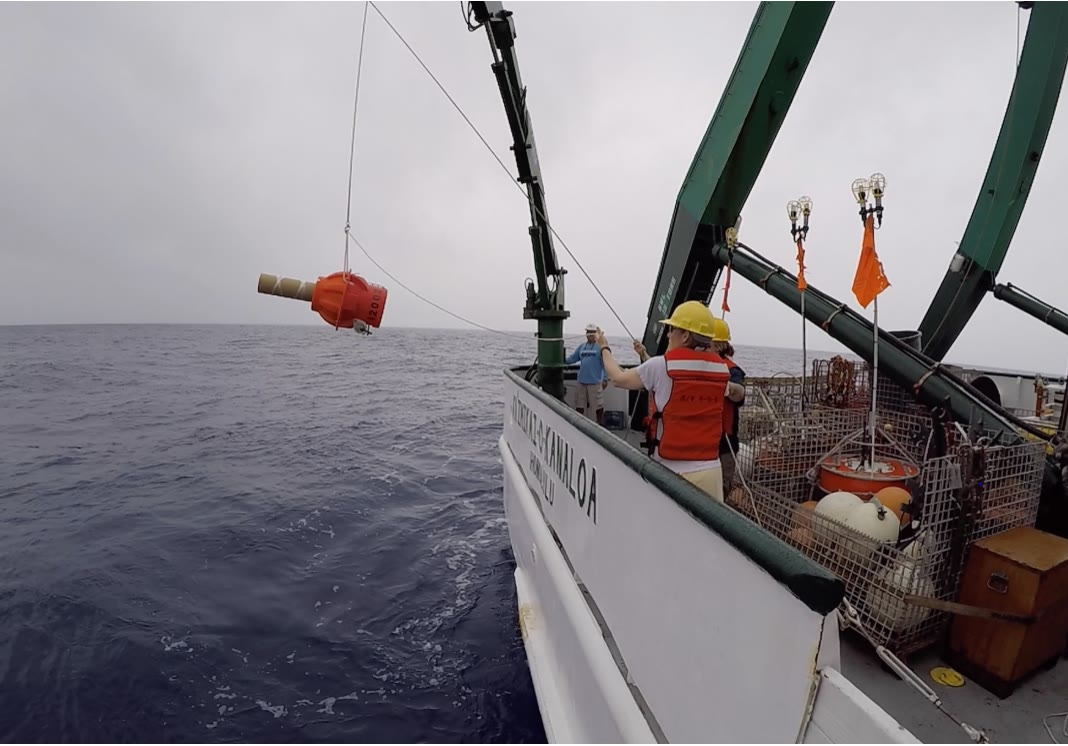
\includegraphics[width=0.6\linewidth]{images/book3/b1-deep-float.jpg}

{\small 一台深海剖面漂浮器（吊在起重机上的橙色仪器）
于 2018 年自科考船上被放入水中；一经释放，它便下沉至工作深度，
并定时上浮以发送数据。（照片：NOAA 摄影师身份不详，
公有领域，经维基共享资源提供。）}
\label{fig:b1:ocean-circulation:float}
\end{omfigure}
% ledger: commons:deep-solo, noaa:argo-25

翻转环流输送热量。向北流动的水温暖，返回时已变冷，
说明其热量已在北方释放给大气。

\begin{proposition}[翻转环流输送的热量]\label{prop:b1:ocean-circulation:heat}
设体积输运 $Q$ 以\omterm{def:b1:fluid-envelopes-structure:potential-temperature}{位温} $\theta_1$ 向北穿过某一纬线，
并以 $\theta_2$ 向南返回，且质量净输运为零，则
该翻转环流向北输送的\omterm{def:b1:heat-budget:heat-flow}{热流}量为
\[
  H = \rho c_p\,Q\,(\theta_1 - \theta_2),
\]
其中 $c_p$ 为海水的比热容。
\end{proposition}
% ledger: teos10:cp0

\begin{proof}
每秒钟，质量 $\rho Q$ 向北穿过，携带热含量 $\rho Q
c_p\theta_1$（以任意温度零点计）；同样的质量向南穿过时，携带热含量
$\rho Q c_p\theta_2$。
净向北通量即二者之差；由于两股质量相等，任意零点相互抵消，
所得结果即为真正的热量输运。
\end{proof}

据 W.~Schmitz 对北大西洋所作的粗略收支估算，墨西哥湾流以 \qty{18}{\celsius} 向北输送
\qty{40}{\sverdrup} 的水体，其中
\qty{14}{\sverdrup} 以 \qty{2}{\celsius} 的深层水向南返回。取 $c_p =
\qty{3992}{J.kg^{-1}.K^{-1}}$，$\rho = \qty{1027}{kg.m^{-3}}$，则该翻转环流
在北纬 \ang{24} 以北输送的热量为 $1027 \times 3992 \times \num{14e6} \times 16 = \qty{0.92e15}{W}$，约
\qty{0.9}{PW}；较为审慎的估算给出 \qty{1.2}{PW}，约占大气与海洋共同向极输送热量的
四分之一。
此热量大部分释放给北大西洋北部上空的空气，
这也是挪威位于北纬 \ang{60}，却远比同\omterm{def:b1:spherical-astronomy:geographic}{纬度}的
格陵兰岛南部温暖的原因之一。
% ledger: stewart:heat-conveyor, rapid:home, teos10:cp0 (computed in calc/ch29.py)

深层环流十分缓慢。若北大西洋下沉的水体
经南极绕极流抵达北太平洋约需一千年，则其平均速率约为 \qty{1}{mm/s}，
比流速计所记录到的多变深层流低约一百倍。
因此，其速度需由示踪剂推断，而非直接测量：
氚由 1950 年代的核试验释放进入大气，半衰期为 12.3 年，
进入深层水形成的北大西洋深处，经过 25 年后仅向南
扩展到北纬 \ang{30} 以南的很小范围，平均速率不足 \qty{1}{mm/s}。
大洋的体积，除以深层水的形成速率，
得到的时间量级与此相同
（见\cref{exo:b1:ocean-circulation:12}）。
% ledger: stewart:deep-circulation, nos:conveyor

南极绕极流连通各大洋盆地。其速度在海底处
仍然很慢，约为 \qty{10}{cm/s}，在其锋面处可达 \qty{50}{cm/s}；但它既深且宽：
在南美洲与南极洲之间的德雷克海峡，一列系泊流速计测得流量为
\qty[uncertainty-mode=separate]{125 \pm
11}{\sverdrup}（发表于 1985 年）；2007 至 2011 年间布设的更密集阵列，
同时测量了近底层的速度，测得 \qty{173.3}{\sverdrup}，
比长期采用的该数值高出 \qty{39}{\percent}。它将深层水
从各大洋输送到其他大洋，并在途中使其混合。
% ledger: stewart:acc, donohue:acc

\begin{dated}{2021}
% ledger: ipcc:amoc-observed, ipcc:amoc-projected
政府间气候变化专门委员会 2021 年的评估依据重建资料认为，
过去 \num{8000} 年间大西洋翻转环流相对稳定（\emph{中等信度}），
其减弱始于 19 世纪末（\emph{中等信度}），
但对 20 世纪内的整体下降，仅有\emph{低信度}。
2000 年代中期至 2010 年代中期直接观测到的减弱（\emph{高信度}），
无法与十年尺度的变率区分开来（\emph{高信度}）。
对于所有排放情景，翻转环流在 21 世纪\emph{很可能}减弱，
但对下降幅度的大小，
仅有\emph{低信度}；认为其在 2100 年前
不会突然崩溃，信度为\emph{中等信度}。
\end{dated}

\section{练习}

\begin{exercise}[$\star$]\label{exo:b1:ocean-circulation:1}
取 $\rho_a = \qty{1.3}{kg.m^{-3}}$，用块体公式及
耶兰德与泰勒的阻力系数。(a)~计算风速为 4、7 与
\qty{15}{m/s} 时的 $C_D$ 与\omterm{def:b1:ocean-circulation:wind-stress}{风应力}。(b)~\omterm{def:b1:ocean-circulation:wind-stress}{风应力}由 7 增至 \qty{15}{m/s} 时，增大到原来的多少倍？
与风速平方之比作比较，并说明差异的原因。
% ledger: stewart:wind-stress, stewart:drag-coefficient
\end{exercise}

\begin{exercise}[$\star$]\label{exo:b1:ocean-circulation:2}
分别给出各情形下\omterm{def:b1:ocean-circulation:ekman}{埃克曼输送}的方向。(a)~向东吹的风，
位于北纬 \ang{45} 处。(b)~来自东北的\omterm{def:b1:atmospheric-circulation:winds}{信风}，位于北纬 \ang{15} 处。
(c)~向东吹的风，位于南纬 \ang{50} 处。(d)~沿非洲南部西海岸、来自南方的风，
位于南纬约 \ang{23} 处。在这四种情形中，哪些输送指向离岸方向？
由此会产生什么结果？
\end{exercise}

\begin{exercise}[$\star$]\label{exo:b1:ocean-circulation:3}
在大西洋北纬 \ang{26.5} 处，2004--2024 年的平均输送为：佛罗里达海峡
\qty{31.7}{\sverdrup}，\omterm{def:b1:ocean-circulation:ekman}{埃克曼输送} \qty{3.5}{\sverdrup}，上层大洋中部
\qty{-17.9}{\sverdrup}；按层计，0--\qty{800}{m} 为 \qty{16.6}{\sverdrup}，
800--\qty{1100}{m} 为 \qty{0.4}{\sverdrup}，1100--\qty{3000}{m} 为 \qty{-12.0}{\sverdrup}，
3000--\qty{5000}{m} 为 \qty{-5.9}{\sverdrup}（向北为正）。(a)~将前三项相加，
并与已发表的翻转环流 \qty{17.1}{\sverdrup} 作比较。(b)~比较
\qty{1100}{m} 以上向北的流量与以下向南的流量。(c)~将
\qty{17.1}{\sverdrup} 换算为立方千米每年，并计算该流量
充满整个海洋体积 \qty{1.3324e9}{km^3} 所需的时间。
% ledger: rapid:transports, charette:ocean-volume
\end{exercise}

\begin{exercise}[$\star$]\label{exo:b1:ocean-circulation:4}
利用埃克曼公式，计算在风速为
\qty{10}{m/s}、\omterm{def:b1:spherical-astronomy:geographic}{纬度}分别为 \ang{15}、\ang{45} 与 \ang{60} 时的埃克曼深度与表层流速，
并给出表层流速占风速的百分比。为什么公式在赤道附近失效？
% ledger: stewart:ekman-constants
\end{exercise}

\begin{exercise}[$\star\star$]\label{exo:b1:ocean-circulation:5}
在大西洋北纬 \ang{11} 处，取平均\omterm{def:b1:ocean-circulation:wind-stress}{风应力}为 \qty{0.07}{Pa}，方向向西，
作用宽度为 \qty{5000}{km}，$\rho = \qty{1027}{kg.m^{-3}}$。
(a)~计算单位米宽的\omterm{def:b1:ocean-circulation:ekman}{埃克曼输送}及其方向。(b)~计算
穿过该断面的总体积输送（以\omterm{def:b1:ocean-circulation:ekman}{斯韦德鲁普}计）。(c)~与
直接测得的输送（$12.0 \pm \qty{5.5}{\sverdrup}$）及由
长期风场计算得到的输送（$13.5 \pm \qty{0.3}{\sverdrup}$）作比较。
% ledger: stewart:ekman-transport
\end{exercise}

\begin{exercise}[$\star\star$]\label{exo:b1:ocean-circulation:6}
沿赤道太平洋，\omterm{def:b1:atmospheric-circulation:winds}{信风}施加的应力为 \qty{0.05}{Pa}，
方向向西。(a)~计算单位米宽的\omterm{def:b1:ocean-circulation:ekman}{埃克曼输送}及其方向，位于
北纬 \ang{2} 与南纬 \ang{2} 处。(b)~假设这两个\omterm{def:b1:spherical-astronomy:geographic}{纬度}所带走的水，
由两\omterm{def:b1:spherical-astronomy:geographic}{纬度}之间的下方补充，计算平均上升速度，
单位为米每天。(c)~定理的公式在赤道本身会如何？
哪个结论依然成立？
\end{exercise}

\begin{exercise}[$\star\star$]\label{exo:b1:ocean-circulation:7}
在\omterm{def:b1:ocean-circulation:gyre}{副热带环流}中，取\omterm{def:b1:ocean-circulation:wind-stress}{风应力}为 \qty{0.06}{Pa}、方向向西，作用于
北纬 \ang{15} 处，以及 \qty{0.12}{Pa}、方向向东，作用于北纬 \ang{40} 处。(a)~计算两处的\omterm{def:b1:ocean-circulation:ekman}{埃克曼输送}
及其方向。(b)~假设两\omterm{def:b1:spherical-astronomy:geographic}{纬度}之间的输送均匀变化，
计算\omterm{def:b1:ocean-circulation:ekman}{埃克曼层}底部的垂向速度，
单位为米每年，并判断其向上还是向下。(c)~在
宽 \qty{5000}{km} 的洋盆中，有多少\omterm{def:b1:ocean-circulation:ekman}{斯韦德鲁普}的水通过该层底部被抽吸？
\end{exercise}

\begin{exercise}[$\star\star$]\label{exo:b1:ocean-circulation:8}
取 $\rho = \qty{1027}{kg.m^{-3}}$ 与 $c_p = \qty{3992}{J.kg^{-1}.K^{-1}}$。
(a)~计算以 \qty{17}{\sverdrup} 向北流动、温度为
\qty{15}{\celsius}、返回时温度为 \qty{3}{\celsius} 的水所输送的向北热量。(b)~与
大西洋翻转环流输送的 \qty{1.2}{PW} 作比较。(c)~若同样的水
在表层沿洋盆东侧向南返回，温度为 \qty{12}{\celsius}，
它将输送多少热量？这说明\omterm{def:b1:ocean-circulation:moc}{深水
形成}的重要性如何？
% ledger: rapid:home, teos10:cp0
\end{exercise}

\begin{exercise}[$\star\star$]\label{exo:b1:ocean-circulation:9}
南大西洋的三种\omterm{def:b1:fluid-envelopes-structure:ts-diagram}{水团}，其\omterm{def:b1:fluid-envelopes-structure:potential-temperature}{位温}与盐度分别为：
南极中层水 \qty{3.3}{\celsius}、34.15；北大西洋
深层水 \qty{4.0}{\celsius}、35.00；南极底层水 \qty{0.4}{\celsius}、
34.67。某深度处的样品具有 $\theta = \qty{2.78}{\celsius}$ 与 $S = 34.731$。
利用\cref{prop:b1:fluid-envelopes-structure:mixing}，求样品中各\omterm{def:b1:fluid-envelopes-structure:ts-diagram}{水团}
所占的比例。
% ledger: stewart:deep-circulation
\end{exercise}

\begin{exercise}[$\star\star\star$]\label{exo:b1:ocean-circulation:10}
取\cref{prop:b1:ocean-circulation:spiral}中的螺旋。(a)~证明 $u$ 与 $v$
满足 $f v + A_z u'' = 0$ 与 $-f u + A_z v'' = 0$。（提示：写出 $u + iv =
V_0\,e^{i\pi/4}\,e^{(1+i)az}$。）(b)~证明应力 $\rho A_z\,\partial\vec
v/\partial z$ 在表面处等于\omterm{def:b1:ocean-circulation:wind-stress}{风应力} $(0, T)$。(c)~计算
输送 $\int_{-\infty}^0 \rho u\,\mathrm dz$ 与 $\int_{-\infty}^0 \rho
v\,\mathrm dz$，并验证它们与
\cref{thm:b1:ocean-circulation:ekman}一致。
\end{exercise}

\begin{exercise}[$\star\star\star$]\label{exo:b1:ocean-circulation:11}
在斯托默尔模型中，\omterm{def:b1:ocean-circulation:wbc}{西边界流}的宽度约为 $R/\beta$，
其中 $R$ 为底部摩擦率，$\beta = \mathrm df/\mathrm dy$ 为
\omterm{def:b1:atmospheric-circulation:coriolis-parameter}{科里奥利参数}沿向北方向的增长率。(a)~证明 $\beta = 2\Omega
\cos\varphi/a_\oplus$，并取地球半径 $a_\oplus = \qty{6371}{km}$，算出北纬 \ang{30} 处的该值。
(b)~取 $R = \qty{e-6}{s^{-1}}$，计算该宽度。(c)~一股
\qty{30}{\sverdrup} 的输送在宽 \qty{5000}{km} 的洋盆内部、上层 \qty{1000}{m} 内向南漂移，
并在同一深度的边界流中向北返回。计算两者的平均速率，
并与墨西哥湾流的速率
\qty{1.8}{m/s} 作比较。
% ledger: stewart:north-atlantic, nos:gulf-stream, earth:Rmean
\end{exercise}

\begin{exercise}[$\star\star\star$]\label{exo:b1:ocean-circulation:12}
海洋的体积为 \qty{1.3324e9}{km^3}，覆盖面积为 \qty{361.84e6}{km^2}。(a)~证明
\qty{1000}{m} 以下的体积至少为 \qty{9.71e8}{km^3}。(b)~北大西洋深层水
约以 \qty{17}{\sverdrup} 的流量形成，南极底层水约以
\qty{9}{\sverdrup} 的流量形成。估算更新 \qty{1000}{m} 以下水体所需的时间，
并与输送带的一千年相比较。(c)~氚的
半衰期为 12.3 年。经过 25 年后，氚输入量中
仍残留的比例是多少？以 \qty{1}{mm/s} 运动的水，在 25 年内能走多远？
% ledger: charette:ocean-volume, stewart:deep-circulation, stewart:acc, rapid:transports
\end{exercise}

\section{问题：一处上升流海岸}

\begin{problem}[{周末问题——北纬 \ang{38} 处海岸上的夏季风}]
\label{pb:b1:ocean-circulation:1}
% values: calc/ch29.py (invented coast; constants from the ledger)
一条南北\omterm{def:b1:geological-maps:attitude}{走向}的笔直海岸位于北纬 \ang{38}，海洋在其西侧。夏季，
一股稳定的 \qty{8}{m/s} 风自北沿海岸吹送，持续数周。该
海岸为虚构，但其数值典型于大洋的东岸。
取 $\Omega = 2\pi/(\qty{23.9345}{h})$，$\rho_a = \qty{1.3}{kg.m^{-3}}$，阻力系数
采用 Yelland 与泰勒的数值，海水的密度 $\rho = \qty{1027}{kg.m^{-3}}$，
及定压比热 $c_p = \qty{3992}{J.kg^{-1}.K^{-1}}$。

\medskip
\noindent\textbf{第一部分——风及其应力。}
\begin{enumerate}
  \item 风朝何方吹？它是沿海岸吹，还是
        垂直于海岸吹？
  \item 计算阻力系数。
  \item 计算\omterm{def:b1:ocean-circulation:wind-stress}{风应力}。
  \item 对风速为 \qty{12}{m/s} 的风，回答同样的两个问题。应力增长了
        多少倍？为何它大于风速平方之比？
  \item 计算北纬 \ang{38} 处的\omterm{def:b1:atmospheric-circulation:coriolis-parameter}{科里奥利参数}。
  \item 以小时为单位计算 $2\pi/f$。为何风须吹一天或更久，
        埃克曼平衡才适用？
\end{enumerate}

\medskip
\noindent\textbf{第二部分——\omterm{def:b1:ocean-circulation:ekman}{埃克曼层}。}
\begin{enumerate}[resume]
  \item \omterm{def:b1:ocean-circulation:ekman}{埃克曼输送}的方向如何？是指向陆地，还是指向开阔海洋？
  \item 计算每米海岸的埃克曼质量输送。
  \item 将其换算为每米的体积输送。
  \item 用埃克曼公式计算埃克曼深度。
  \item 以 \unit{cm/s} 为单位，计算该层内的平均离岸速度。
  \item 用埃克曼公式计算表层洋流及其方向。漂流浮标的测量结果
        反而对其速率给出了怎样的提示？
\end{enumerate}

\medskip
\noindent\textbf{第三部分——海岸\omterm{def:b1:ocean-circulation:upwelling}{上升流}。}
\begin{enumerate}[resume]
  \item 借助竖直剖面示意图，说明离岸输送的水
        来自何处。
  \item 计算沿海岸每千米每天上升的水体积。
  \item 设水体沿海岸穿过宽 \qty{20}{km} 的带状区域上升。
        计算平均上升速度，分别以 \unit{m/s} 和每天若干米为单位。
  \item 水以此速度从\omterm{def:b1:ocean-circulation:ekman}{埃克曼层}底部升至
        表面需要多长时间？
  \item 上升的水在 \qty{12}{\celsius} 时到达表面，而离岸的
        开阔海水为 \qty{18}{\celsius}。海风将温暖
        湿润的离岸空气带到这片水面上方。近地面的空气将
        发生怎样的变化？海岸随之会出现什么天气？
  \item 为何此类海岸鱼类资源丰富？
  \item 秋季风向转变，连续一周自南向吹。输送情况
        及海岸处的水体会发生什么变化？
\end{enumerate}

\medskip
\noindent\textbf{第四部分——其他海岸与总输送。}
\begin{enumerate}[resume]
  \item 应力不变时，计算北纬 \ang{20} 处每米的\omterm{def:b1:ocean-circulation:ekman}{埃克曼输送}，
        并与北纬 \ang{38} 处的结果相比较。
  \item 在南部非洲西海岸、靠近南纬 \ang{23} 处，哪种风向
        驱动\omterm{def:b1:ocean-circulation:upwelling}{上升流}？与本题的海岸相比较，情况如何？
  \item 若在北纬 \ang{38} 处风速为 \qty{5}{m/s} 而非 \qty{8}{m/s}，计算
        应力及每米\omterm{def:b1:ocean-circulation:ekman}{埃克曼输送}，并求它们与
        第~8 题相应结果之比。
  \item 上升的水在向离岸漂移时升温 \qty{6}{\celsius}。计算
        每秒每米海岸所吸收的热量，再求沿
        \qty{1000}{km} 海岸的总量。
  \item 这样的海岸需要多长，才能上升的水量与墨西哥湾流
        经佛罗里达海峡的输送量 \qty{31.7}{\sverdrup} 相等？
  \item 以\omterm{def:b1:ocean-circulation:ekman}{斯韦德鲁普}为单位，沿此 \qty{1000}{km} 的
        海岸上升的水体积是多少？
\end{enumerate}
\end{problem}
